\documentclass[10pt,conference,letterpaper]{IEEEtran}
\usepackage{graphicx,amsmath,booktabs,url}
\graphicspath{{figures/}}
\newcommand{\head}[1]{\subsection*{#1}}
\newcommand{\pic}[2]{\begin{center}\includegraphics[width=\linewidth]{#1}\\[-1pt]{\footnotesize #2}\end{center}}
\newcommand{\spread}[3]{\clearpage\twocolumn[{\centering{\Large\bfseries #1\par}\vspace{4pt}{\normalsize #2\par}\vspace{9pt}#3\vspace{8pt}}]}
\newcommand{\code}[1]{\texttt{#1}}
\begin{document}
\title{From Five Canny Stages to a Cache-Local SIMD Pipeline}
\author{\IEEEauthorblockN{Pranav Kumara, Aman Gupta, and Krish Patel}
\IEEEauthorblockA{Team 11 \hspace{1em} 18-645: How to Write Fast Code \hspace{1em} Carnegie Mellon University}}
\maketitle\pagestyle{plain}\thispagestyle{plain}
\begin{abstract}
On a native $3840\times2160$ photograph, our five-stage SIMD implementation on eight physical cores took 14.97 ms. Keeping Sobel intermediates local and classifying directly in non-maximum suppression reduced latency to 9.52 ms. Feeding those tiles from a local Gaussian ring reduced it to 4.57 ms. All three implementations matched the fixed-point scalar labels and edges exactly. We explain this $3.28\times$ same-thread improvement alongside independent measurements of the production kernels with L1-resident data. Extra independent groups helped only within limits set by instruction mix, register lifetimes and the consumer's access pattern.
\end{abstract}
\section{What improved?}
Canny converts a grayscale image into an edge map. Smoothing reduces noise. Sobel measures changes in brightness. Non-maximum suppression (NMS) thins ridges, classification labels potential edges, and hysteresis follows connected edges. In a straight implementation, each pass writes its result to memory and the next pass reads it back. This organization is easy to validate. On a large image the intermediate maps exceed private cache capacity.
\head{Two useful comparisons}
To ask what fusion buys, compare two optimized implementations on the same input and worker count. On eight cores the fully fused 4K run was $14.974/4.566=3.28\times$ faster than five SIMD passes. To ask how much the complete project buys over scalar code, use the matched single-thread scalar oracle. At 4K it took 260.47 ms in the eight-worker series, a $57.0\times$ overall ratio that includes both vectorization and parallelism.
\pic{frames}{Whole-frame latency; labels are milliseconds. Scalar values here come from the one-worker run series. File I/O is excluded.}
\head{What the final design emits}
The filtering stage emits one byte of labels per pixel. Magnitude and gradient planes are temporary tile data. Hysteresis consumes the labels and writes a byte edge map. Queue work varies with the scene, so a per-frame latency complements the regular kernels' throughputs.
\head{Which comparisons answer the midterm comments?}
The report first follows one pixel through the pipeline, then asks three experimentally separate questions. Does a proposed instruction change compute the same answer? Which hardware resource sets an optimistic lower bound on cycles? What happened to a warmed kernel and to a real frame when we changed that instruction schedule? Results on a photograph answer the application question; the dedicated L1 runs answer the kernel question.
\head{Reading the units}
An integer lane-op is an explicitly counted operation on one SIMD lane. Each kernel states which operations enter that numerator. A floating-point operation counts only floating-point arithmetic. The final pixel path uses integer arithmetic. We report floating-point counter results for the fused workload and an actual GFLOP/s benchmark for the historical FP32 Gaussian. Page 9 explains the distinction.
\spread{2. Follow an edge through five stages}{A $3\times3$ Sobel window reads a small region of the smoothed image.}{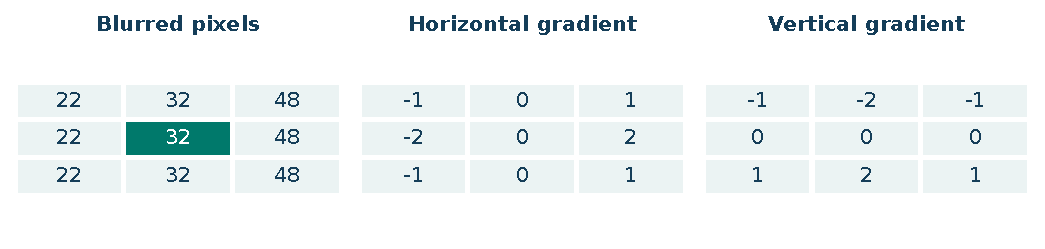
\includegraphics[width=.92\textwidth]{sobel-masks}}
\head{A worked pixel}
Consider a vertical boundary where every row has intensity 20 to the left and 60 to the right. After smoothing, three adjacent columns near the boundary are 22, 32 and 48. Their values are the same on each row. The middle grid above gives $G_x=(48-22)+2(48-22)+(48-22)=104$. The bottom and top weighted sums both equal $22+2(32)+48=134$, so $G_y=0$. The production magnitude is $|104|+|0|=104$.
\head{Which neighbor wins?}
The local magnitudes to the left, center and right are 48, 104 and 104. The gradient points horizontally. NMS requires the center to exceed the left and to equal or exceed the right. The center survives; the next pixel loses its tie on the left. The thresholds 60 and 120 give the surviving center a weak label. It becomes an edge only if a path through other candidate pixels reaches a strong one.
\head{Five stages and their dependencies}
Gaussian, Sobel and NMS are neighborhood calculations. With input rows ready, their output centers are independent. Thresholding is pointwise. Hysteresis differs: promoting one weak pixel can enable a later promotion. This difference determines our fusion boundary.
\newpage
\head{How the buffers change}
\begin{verbatim}
Separate SIMD stages
 image -> full blur
       -> full M, Gx, Gy
       -> full suppressed M
       -> labels -> edges

Partial fusion
 image -> full blur
       -> [local Sobel, NMS, labels]
       -> labels -> edges

Final tiles
 image -> [Gaussian ring
           -> local Sobel planes
           -> NMS + thresholds]
       -> labels -> edges
\end{verbatim}
Tile-local arrays still have loads and stores. Their advantage is a short distance in time between producing a value and consuming it.
\head{Numerical contract}
The final driver uses $\sigma=1$, a reflected input for the five-tap Gaussian, clamped blurred coordinates for Sobel, and a zero NMS image border. The midterm Gaussian example used $\sigma=1.4$. The scalar oracle in this comparison uses the final weights, rounding, tie rule and thresholds. A float/square-root variant would require its own reference and threshold calibration.
\head{Correctness gate}
The driver builds scalar labels and a scalar edge map. It compares both full arrays against each timed variant. Matching labels checks suppression and threshold boundary behavior before connectivity can conceal a mismatch.
\spread{3. Gaussian blur: what do the functions do?}{Separate the weighted arithmetic from the cost of acquiring neighboring pixels.}{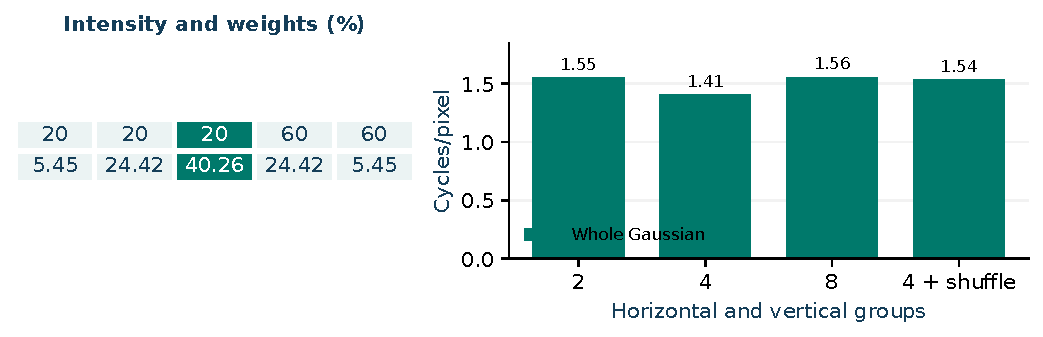
\includegraphics[width=.70\textwidth]{gaussian}}
\head{A five-tap function, applied twice}
$M(x,c)=\lfloor(xc+16384)/32768\rfloor$ is a signed, rounded fixed-point product. It maps to \code{vpmulhrsw}. Each input byte $I$ is expanded to $64I$. For $\sigma=1$ the symmetric Q15 weights from left to right are 1785, 8002, 13193, 8002, 1785. Pairing the equal weights needs three products per axis. The horizontal result stays scaled by 64. The vertical pass applies the same function down a column, then rounds $(Y+32)/64$ to an output byte.
\head{One output row at a time}
Five horizontally filtered rows occupy a ring. The vertical pass consumes those five rows. Before the next output, the expired slot receives one newly filtered input row. A 256-bit AVX2 vector holds sixteen of the intermediate 16-bit values; each lane computes its own center.
\head{Why a shuffle cannot do the multiply}
A shuffle can put the correct neighbor in a lane. It cannot apply a coefficient. The alternative worth measuring is to build shifted neighbor vectors from aligned loads with shuffles, then apply the same three products. The resulting bytes must match the original kernel.
\newpage
\head{Why four groups was a hypothesis}
On this CPU two eligible multiply micro-ops can start per cycle and a dependent consumer waits five cycles. Sustaining this multiply rate calls for roughly ten independent products in flight. Four groups supply twelve candidate products. Two per group depend on a pair addition. Loads, shared ports and finite registers determine when those candidates become ready.
\head{Why measure separate phases?}
Counting three multiplies and four adds per pixel per axis gives 14 useful lane-ops/pixel. An arithmetic-only upper bound is $3\times16=48$ lane-ops/cycle if the instruction mix can use the three ports. The implementation runs expansion, horizontal and vertical/output loops in sequence. In the 64-pixel compiled-body model expansion needs at least four cycles, horizontal needs 14 (28 load services over two ports, assuming half the shifted loads split), and vertical/output needs 13.5 (54 allocation slots at four/cycle). Together $31.5/64=0.492$ cycles/pixel gives a useful rate ceiling of $14/0.492=28.44$. Standalone image borders and ring fill can lower achieved throughput further.
\head{What happens on hardware}
In the initial pinned run, the four-group Gaussian on a warmed $256\times24$ image (16,000 bytes touched) measured 0.872 cycles/pixel. With heavier shared-host load, a repeated comparison measured 1.405, or 9.97 useful integer lane-ops/cycle. Two and eight groups took 1.553 and 1.558 on that same repeated workload. The eight-group horizontal loop spilled vector temporaries. The four-group shuffle variant took 1.538 cycles/pixel; the added shuffle demand outweighed its reduced shifted-load traffic. The arithmetic peak alone cannot explain either the slowdown or the change between runs. We retained four groups.

The measured horizontal and vertical row phases were 0.398 and 0.506 cycles/pixel. In a separate non-multiplexed profile, 0.0645\% of the counted retired Gaussian loads missed L1. The paired whole-image rate is 35\% of the implementation ceiling and 21\% of the arithmetic ceiling. In the shuffle design at least six p5 shuffles/group compete with an original load estimate of 3.5 cycles/group. Shorter individual shuffle latency alone gives no throughput advantage.

\spread{4. Sobel: choose the register tile}{A sliding window computes ten gradient rows before non-maximum suppression consumes the center eight.}{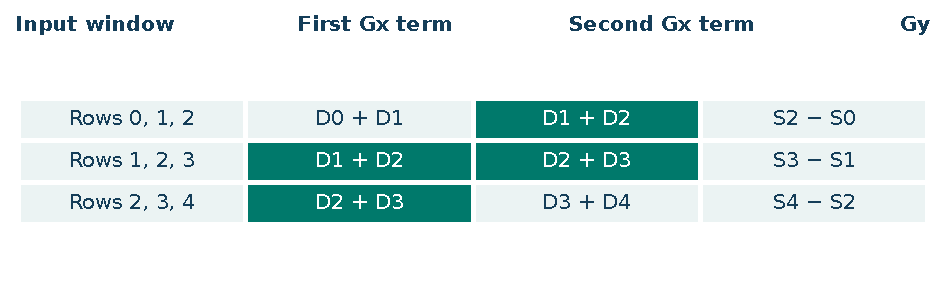
\includegraphics[width=.86\textwidth]{sliding}}
\head{Two values per input row}
For each row compute $D=R-L$ and $S=L+2C+R$. The code forms $T=R+C$ and $S=2T-D$, which gives the same sum. For a vertical window,
\[
 G_x=D_t+2D_m+D_b,\qquad G_y=S_b-S_t.
\]
Writing $G_x=(D_t+D_m)+(D_m+D_b)$ exposes an adjacent-row sum that becomes the first term of the next output. Each time we slide down, we bring in one new row. We store magnitude and both gradients for NMS.
\head{What the 10 by 16 name means}
Ten rows of output, each sixteen int16 lanes wide, form 160 centers. One $10\times16$ tile needs a $12\times18$ rectangle of blurred input. The six-row standalone driver from the midterm did different work. We updated the driver to compile and link the production ten-row object and check all three planes against scalar Sobel.
\head{Count the vector instructions}
Green cells in the diagram show adjacent sums carried into the next output. The final loop listing contains 55 packed adds, 34 packed subtracts, and 20 packed absolute values. Thus the numerator is $(55+34+20)16=1744$ lane-ops per 160 centers, or 10.9 per pixel. This is the executed gradient/magnitude arithmetic count for this tile, including row setup.
\newpage
\head{Identify a limiting resource}
The adds and subtracts can distribute over ports 0, 1 and 5; the 20 absolute values fit within their eligible execution capacity. Evenly distributing 109 arithmetic micro-ops gives at least $109/3=36.33$ cycles per tile, so the vector arithmetic ceiling is $1744/36.33=48.0$ integer lane-ops/cycle. Thirty vector stores need at least 30 store-data cycles; 36 input loads need at least 18 ideal load cycles before splits.
\head{Why the ports can still wait}
The assembly has 155 instructions in its loop including the compare and branch. With one fused compare/branch and an optimistic four allocation slots per cycle, its allocation floor is about $154/4=38.5$ cycles. This is a second, tighter optimistic ceiling, roughly 45.3 lane-ops/cycle. Neither floor predicts every real cycle. Loop calls, dependencies, scheduling, addresses and cache-line splits can all consume time. Measured port activity appears on page 6.
\head{Which size was useful?}
A 128-column strip touches 11,520 bytes of cache lines for the ten-row loop. One group measured 32.5 lane-ops/cycle, about 68\% of the vector ceiling. Two and four groups improved the median on that width. At width 256 four groups regressed. The four-group assembly acquired 40 vector stack references per unrolled loop; the single-group version had none. Comparing the actual frame establishes which change deserves production use.
\spread{5. Fusing suppression with thresholding}{Directional neighbor selection and class labeling share a single register loop.}{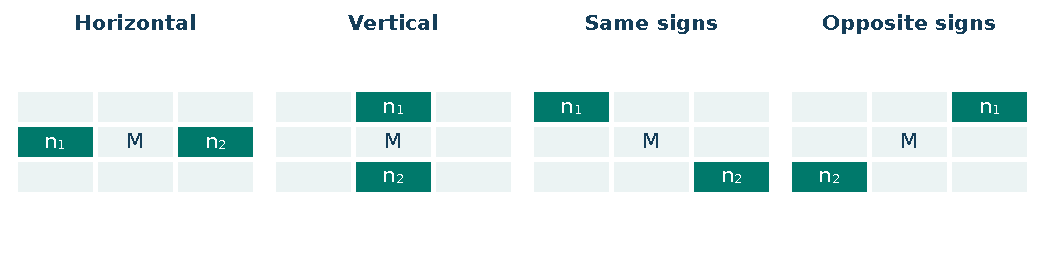
\includegraphics[width=.87\textwidth]{directions}}
\head{Recover direction from the gradients}
Let $a=|G_x|$, $b=|G_y|$, and $t=\lfloor27146a/65536\rfloor$. The multiplier approximates $\tan(22.5^\circ)$. If $b\le t$, use the left and right magnitudes. If $b>2a+t$, use the magnitudes above and below. Otherwise the gradients' sign agreement selects one of the diagonals. Signed integer ordering and the strict/weak tie convention are part of the algorithm.
\head{Compare once}
For integer magnitudes, $m>n_1$ and $m\ge n_2$ is equivalent to $m>\max(n_1,n_2-1)$. The vector loop constructs the four directional limits, selects the right limit with masks, and compares the center once. Two more compares and arithmetic on their masks form a byte label. The pipeline writes no full suppressed-magnitude image.
\head{Loop size and counted work}
The production loop handles two output rows and four groups of sixteen columns: 128 pixels. Direction, suppression and classification contribute 26 word-lane operations per pixel or 3328 per loop. Loads, stores, address math, extraction and byte packing do not enter this numerator, but the corresponding resources still enter the denominator.
\newpage
\head{Find the busiest port group}
The linked loop contains 208 counted vector instructions, including 24 variable blends. Each blend costs two execution micro-ops. Eight upper-half extracts and eight byte packs also use execution capacity. Thus at least $(208+24+8+8)/3=82.67$ cycles are required across ports 0, 1 and 5. Before splits the 88 vector loads need at least 44 load cycles, and eight stores need at least eight store-data cycles. The 16 shuffle-only operations fit on port 5 and the restricted compares, maxima, shifts, absolute values and multiplies fit on ports 0/1. No single exclusive instruction takes 82.67 cycles. The busy resource is their combined service capacity. The resulting ideal is $3328/82.67=40.26$ integer lane-ops/cycle.
\head{What the verified driver saw}
At width 128 the four-group loop measured 0.854 cycles/pixel, or 30.43 lane-ops/cycle and 75.6\% of its arithmetic ceiling. The driver compares exact byte labels across 400 fills including ties, opposite signs, small magnitudes and threshold crossings. Inputs, output and halos touched 2624 bytes in this run.
\head{One algebraic alternative}
For nonnegative thresholds, a candidate can produce a label by gating on $m>\max(\mathrm{limit},60)$ and returning either one or two depending on $m>120$. In an alternating L1 comparison this changed 0.858 to 0.813 cycles/pixel, about $1.055\times$. Compare candidates by cycles/pixel: their instruction numerators differ.
\spread{6. Are we filling the execution ports?}{A pinned-core counter experiment on the same warmed 128-column input as the latency benchmark.}{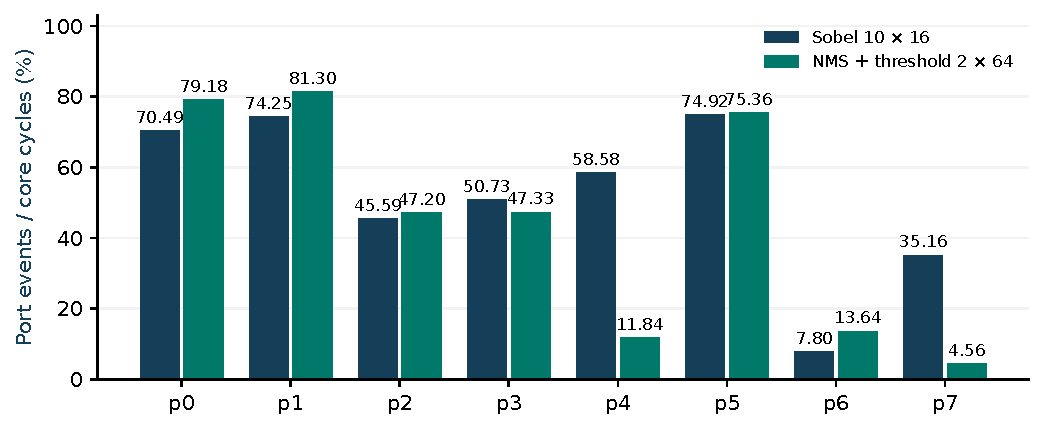
\includegraphics[width=.87\textwidth]{ports}}
\head{The denominator matters}
The chart above shows per-port dispatch events divided by user core cycles. We counted each port in a separate repeat to avoid multiplexing. Kernel calls, short-loop overhead and counter reads are included. The bars are diagnostic averages, not a cycle-by-cycle schedule. Counters cannot tell us which dependency caused every unused slot.
\head{Sobel}
Dispatch events per core cycle for ports 0, 1 and 5 were about 70\%, 74\% and 75\%; the measured retirement rate was 2.97 slots per cycle out of four. This is compatible with the static prediction that arithmetic, allocation and thirty vector stores all matter. It does not demonstrate a saturated individual port. The simple single-group loop avoids vector stack traffic and leaves room for the out-of-order scheduler to overlap independent rows.
\head{NMS and classification}
Corresponding rates were 79\%, 81\% and 75\%, with 2.87 retired slots per cycle. The 24 blends in the loop add dispatch demand beyond the instruction count. Loads enter on separate ports but folded operands can use both load and arithmetic resources. Calling the five-cycle multiply the sole bottleneck would ignore the compares, blends and packs in the same loop.
\newpage
\head{Is it really an L1 test?}
We pin to CPU 10, warm identical strips repeatedly, and count actual distinct 64-byte lines touched by every input, output and halo. Unused address gaps between fixed-stride planes do not consume cache lines. Both working sets fit within the 32 KiB L1D. At width 128, Sobel recorded about 0.00055 L1D replacements per cycle and fused NMS fewer than 0.00002. Replacements count cache-line turnover rather than individual missing load instructions.
\head{Capacity alone fooled us}
At width 256, Sobel still touched only 22,272 bytes, yet the single-group run saw about 0.026 replacements per cycle. Strides, set conflicts, alignment and other thread activity can matter even if the sum of buffer sizes fits. This observation motivated a second, smaller measurement; it does not isolate a single cause. The production 320-column tile has roughly 41 KiB of worker scratch. Its performance belongs in an image benchmark.
\head{Assumptions behind a port bound}
We assume ready independent inputs, steady repeated work and feasible port assignment on Cascade Lake. For ports operating concurrently take the maximum demand/capacity, not the sum of instruction latencies. Add separate phase floors when one loop must finish before the next phase starts. Dependencies, front-end limits, address generation, splits, cache and loop boundaries can reduce the achieved rate. Our ALU percentages use the arithmetic-port ceiling consistently.
\spread{7. How much independent work helps?}{Group count varies inside the compiled loop; image width, arithmetic, outputs and compiler flags stay fixed.}{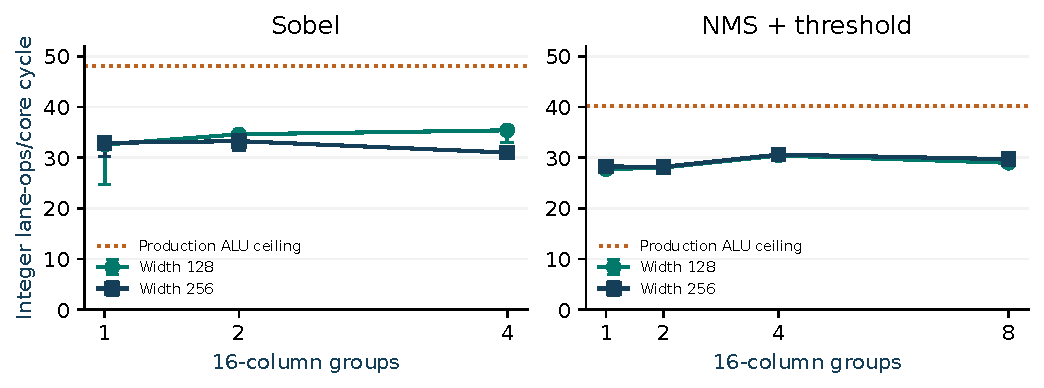
\includegraphics[width=.9\textwidth]{groups}}
\head{Read the experiment}
Each point uses fourteen timed trials, two passes through the variants in opposite orders. Each trial repeats one warmed call 30,000 times. The error bars show the interquartile range. Each output center contains a fixed amount of algorithmic work in a group sweep. We time the candidate only after an exact scalar check.
\head{Sobel changes with width}
Width 128 yielded 0.335, 0.315 and 0.308 cycles/pixel at one, two and four groups. The one-group interquartile range was 0.318--0.442, so the first two distributions overlap. At width 256 the same sequence was 0.331, 0.328 and 0.352. The larger loop also increases hot instructions and register pressure. A higher observed rate on one strip does not establish a better frame kernel.
\head{NMS has an interior optimum here}
On width 128 the one-, two-, four- and eight-group rates were 0.938, 0.926, 0.854 and 0.897 cycles/pixel. Four versus one gives about $1.10\times$. Width 256 also favored four. The eight-group body roughly doubles the instruction footprint relative to four, even though neither has vector stack operands in its hot loop. These data support four groups empirically; they do not establish that every idle cycle is an instruction-cache stall.
\newpage
\head{A resource floor leads to an experiment}
The Sobel group sweep tests a tradeoff between independent work and register capacity. In NMS, the simpler label expression tests whether the arithmetic port mix can be improved while retaining asymmetric ties. For Gaussian, shifted loads versus shuffled lanes changes which hardware resource supplies neighbors. These comparisons all keep the fixed-point outputs and thresholds unchanged.
\head{Test at the consumer boundary}
The microbenchmark measures one hot call. In the tiled pipeline the same worker first constructs Gaussian rows, writes Sobel planes, performs NMS, and interacts with shared caches. The NMS label buffer is copied to its final row, and the hysteresis pass may dominate. We therefore also tested the two-group Sobel and the alternate label expression, separately and together, in the linked application.
\head{Integration decision}
On eight workers the repeat 4K medians were 4.617 ms for the shipped loop, 4.810 for the new label expression, 4.681 for two-group Sobel and 5.124 for both changes. At 1080p the corresponding numbers were 0.874, 0.867, 0.869 and 1.102. For 4K at eight cores the median of within-round gate/original ratios was 0.998, essentially tied. Pooled one-core frame results changed direction with image size. Some batch rankings flipped; the earlier eight-core sweep had extreme outliers under host contention. We retain the production schedule. The $1.055\times$ isolated NMS improvement remains a reproducible experiment rather than a claimed frame speedup.

\spread{8. From threshold labels to connected edges}{Classifying a pixel is independent; establishing connectivity can require following a long path.}{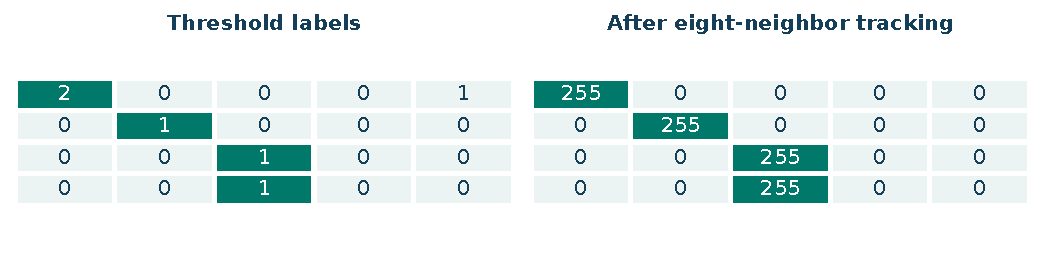
\includegraphics[width=.86\textwidth]{connectivity}}
\head{Threshold math}
For a retained magnitude $m$, $[m>60]+[m>120]$ gives 0 for rejected, 1 for weak and 2 for strong. A suppressed center receives 0. Strict thresholds matter at exactly 60 and 120. In the final loop the result is packed from words to bytes. This keeps full-frame label traffic to one byte per pixel.
\head{Hysteresis math}
Let $S$ contain all strong labels and $W$ all weak ones. Starting with $E_0=S$, repeatedly compute
\[
 E_{k+1}=E_k\cup\{w\in W:\ N_8(w)\cap E_k\ne\emptyset\}.
\]
Stop when no new member joins. Emit 255 for retained pixels and zero elsewhere. In the image above the diagonal weak pixels join the strong component; the isolated one in the upper right is dropped.
\head{Use SIMD where the work is regular}
A YMM register can inspect 32 byte labels. SIMD identifies seeds adjacent to strong pixels; extracting mask bits gives a frontier. The queue then visits newly reachable pixels. Tracking work changes with the number of weak pixels and the shape of their connected components. A seed-free vector scan measures just that first operation.
\newpage
\head{L1 observations}
The historical standalone threshold consumes 32-bit squared magnitudes; the current fused stage consumes 16-bit L1 magnitudes. The separate 64-pixel threshold loop needs eight port-5 pack/permutation operations, giving an ideal eight pixels/cycle. Counting four comparison/classification operations per pixel gives 32 useful lane-ops/cycle on that convention. At width 512, unrolling to 128 outputs reached 0.215 cycles/pixel (18.6 useful ops/cycle), versus 0.309 for 64. Production thresholds stay inside NMS, whose output contract and instruction mix differ.
\head{Independent scan versus dependent queue}
For the exact 32-pixel scan, 21 modeled load-port service units and two load ports give $320/(21/2)=30.5$ byte lane-ops/cycle under the stated split assumption. It reached 17.29 (57\%). The exact scan touched 6,740 bytes; ports 2 and 3 had the highest dispatch rates (0.459 and 0.443 per cycle). Pairing two scan rows improved the seed-free exact-scan median from 0.578 to 0.515 cycles/pixel. On a $258\times8$ slab, pairing improved sparse tracking from 3.496 to 2.753, but regressed dense tracking from 54.679 to 60.086. The queues contained 18 versus 1129 entries. The older 4-row seed predictor has a load service floor of $27/(2\times128)=0.1055$ cycles/pixel; it has a different output contract. A fixed per-pixel arithmetic ceiling is inappropriate for complete queue traversal.

\head{Why the final queue uses the zero border}
NMS fixes the image side columns to zero. A queued center is interior in $x$, so its left and right neighbors exist. For adjacent rows the kernel tests the slab ends once and uses fixed offsets for the neighbors. This removes per-popped-pixel integer division for recovering coordinates. The generic boundary-aware entry point is still used when the caller cannot guarantee the zero border.
\head{Why stop fusion at labels?}
Tiles suffice for local neighborhoods in all previous stages. A weak path may cross several tile boundaries. Letting each worker finalize its own tile in isolation would break it. One complete byte-label map and explicit seam propagation make the result independent of worker boundaries.
\spread{9. What fusion saves on a real image}{All three schedules use the same thresholds, fixed-point arithmetic, scalar oracle and number of workers.}{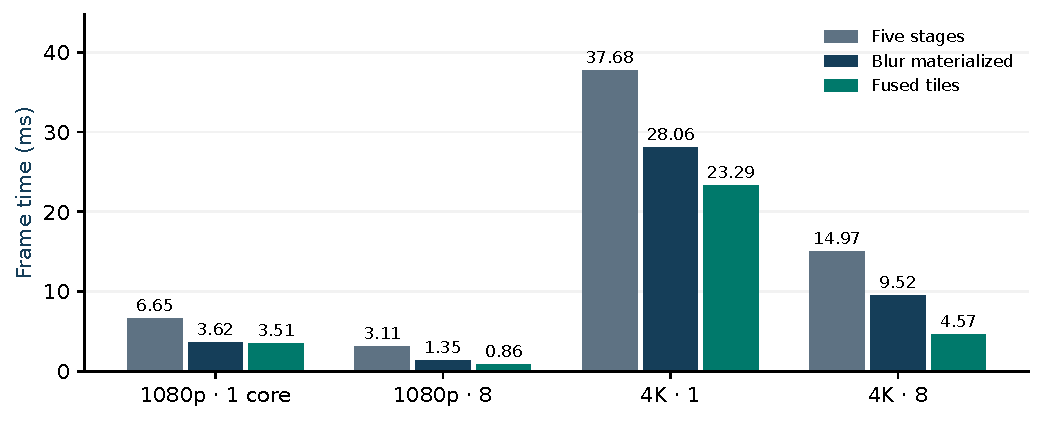
\includegraphics[width=.9\textwidth]{fusion}}
\head{Baseline and controls}
Five separate SIMD stages materialize blur, gradients and magnitude, suppressed magnitudes, labels and edges. The comparison driver explicitly packs full-frame rows for Sobel's fixed-stride interface. The partially fused schedule materializes Gaussian, then keeps the Sobel planes local and classifies inside NMS. The final schedule generates blurred rows locally as well. The separate-to-partial change includes packing, copy, allocation and barrier differences required by these implementations.
\head{Native photography}
On one worker the 4K sequence is 37.68, 28.06 and 23.29 ms. On eight it is 14.97, 9.52 and 4.57 ms. On the 1080p portrait the one-core Gaussian-fusion increment is smaller: 3.62 to 3.51 ms, with overlapping individual timing ranges. Each configuration has 33 trials across three rotated batches. Both labels and final edges matched for all 396 timed runs.
\head{Watch the hierarchy}
For 32 warmed native 4K calls on one pinned worker, retired loads that missed L1 per pixel fell from 0.1934 to 0.1515 to 0.0581. Fully fused versus separate is a 70\% drop. Instructions increased from 9.39 to 10.66 per pixel, while cycles decreased from 13.70 to about 8.45. Extra work on halos can pay when it shortens the trip to the consumer.
\newpage
\head{FLOPs for the fused workload}
There are zero floating-point arithmetic operations in the timed pixel algorithm; its pixel-algorithm throughput in GFLOP/s is zero. At 4K the eight-worker final schedule instead delivers $8{,}294{,}400/0.004566=1.82$ billion pixels/s. We also checked the actual workload with hardware FP events. All packed FP32 and FP64 widths and scalar FP32 were zero. There were 352 scalar-double arithmetic counts over 32 frames, or 11/frame, consistent with timing bookkeeping. Gaussian coefficient generation ran before timing.
\head{An actual FP benchmark}
The original scalar FP32 Gaussian uses a direct $5\times5$ weighted sum: 25 multiplies and 25 accumulator additions per pixel. Using that tap-FLOP convention, one $1920\times1080$ frame contains 103.68 million FLOPs. A median of 250.383 ms gives \textbf{0.414 GFLOP/s} on one pinned core. The stage timer includes output quantization; the numerator excludes it, address arithmetic and coefficient generation. This historical FP implementation is distinct from the matched fixed-point baseline used to calculate the fusion speedup.
\head{Image dependence}
The 1080p portrait and 4K Apollo photograph have different edge content. Compare schedules within a given photograph. To isolate resolution as an independent variable, repeat with the same scene at several resolutions and report how many weak candidates enter the queue.
\spread{10. Parallelization, limits, and next experiments}{Spatial independence enables static filtering tiles; irregular connectivity requires reconciliation.}{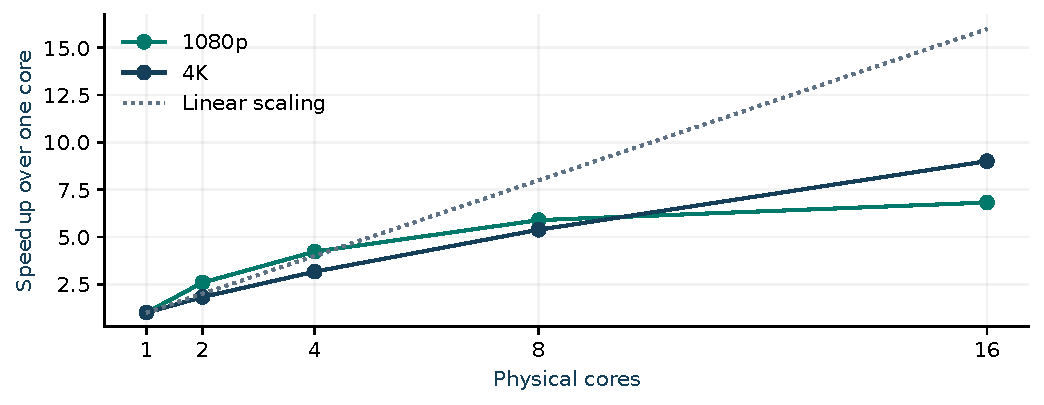
\includegraphics[width=.83\textwidth]{scaling}}
\head{Which rows belong to a worker?}
OpenMP statically assigns independent up-to-$64\times320$ output rectangles. Each worker owns its Gaussian ring, blurred rows and three gradient planes. Across the horizontal axis each SIMD group reads consecutive pixels. Within a 64-row band the worker produces eight useful NMS rows per ten gradient rows and carries four blurred rows to the next block. Rounded widths provide halos and safe SIMD tails; only valid labels are copied to the image.
\head{Where synchronization belongs}
After label generation and border clearing, each worker owns a disjoint horizontal tracking slab. All local queues finish at a barrier. Workers examine stable neighboring edge rows, collect unresolved seam candidates and append to a shared frontier. A final queue connects components crossing multiple slabs. This sequence explains why more cores can eventually expose a serial cost.
\head{Strong scaling}
In the archived final-build sweep the same native 4K photo took 24.63, 13.53, 7.79, 4.58 and 2.735 ms on 1, 2, 4, 8 and 16 physical cores. At 16 cores this is $9.0\times$ speedup, or 56\% parallel efficiency. The 16-worker run spans both sockets; changing memory placement, clock rates, load balance and synchronization contribute uncertainty. The earlier scaling sweep and new fusion comparison are separate measured series.
\newpage
\head{Future directions}
(1) Log the number of queued pixels and elapsed time per slab on a representative image set. If a few dense slabs account for the tail, test smaller ownership regions and measure the extra reconciliation cost. (2) Test stripe width and plane padding together, measuring L1 replacements as well as frame latency. (3) A Halide version could express the same fixed-point formulas and vary producer placement using \code{compute\_at}, tiling and vectorization. Preserve rounding, ties, borders and connectivity and compare against this oracle before comparing schedules. The scheduling model is documented in~\cite{halide}. Halide was optional and has no measured result here.
\head{Reproduction and sources}
ECE024 is a dual-socket Intel Xeon Silver 4208 (Cascade Lake), eight physical cores/socket, two hardware threads/core, 32 KiB L1D and 1 MiB L2/core. The final algorithm follows the kernel, cache and parallel design procedure in~\cite{course}; port eligibility and PMU events use~\cite{peak,pmu}. GCC 8.5 and the repository Makefile specify vectorization, ISA and scheduling flags. AVX2 supplies the regular kernels; the hysteresis seed scan also uses AVX-512VL ternary logic on YMM registers. Run \code{make check} and \code{make fusion FUSION\_IMAGE=noise}. The accompanying walkthrough lists the exact L1, group-sweep, full-frame, profiler and FP commands. Raw trials, compiler-generated disassemblies and the group-count experiments accompany the sources.
\footnotesize
\begin{thebibliography}{6}
\bibitem{course} T. M. Low, CMU 18-645, \emph{Kernels; SIMD; Benchmarking; Wrapping Up Sequential Design; Design for Caches; Explicit Parallelism}, Fall 2026. Especially Wrapping Up, pp. 3--6, and SIMD, pp. 8--12.
\bibitem{peak} A. Abel and J. Reineke, ``uops.info: Characterizing Latency, Throughput, and Port Usage of Instructions,'' ASPLOS, 2019. Cascade Lake instruction entries, \url{https://uops.info}.
\bibitem{pmu} Intel, Performance Monitoring Events, Cascade Lake-X, \url{https://perfmon-events.intel.com/}.
\bibitem{halide} Halide, Tutorial Lesson 8, producer and consumer scheduling, \url{https://halide-lang.org/tutorials/}.
\end{thebibliography}
\end{document}
